\lstdefinestyle{mystyle}{
  basicstyle=\ttfamily,
  breakatwhitespace=false,
  breaklines=true,
  keepspaces=true,
}

\chapter{Gin × Neo4j × Docker で最短経路を返すAPIサーバを建てる}
\section{はじめに}
このセクションでは、現在最もメジャーなグラフDBであるNeo4jとGitHubでも多くのスターを獲得しているGo言語のWebフレームワーク、Ginを用いて
APIサーバーを構築していきます。また、実行環境統一のためDockerを用います。

\section{今回扱うデータの図}
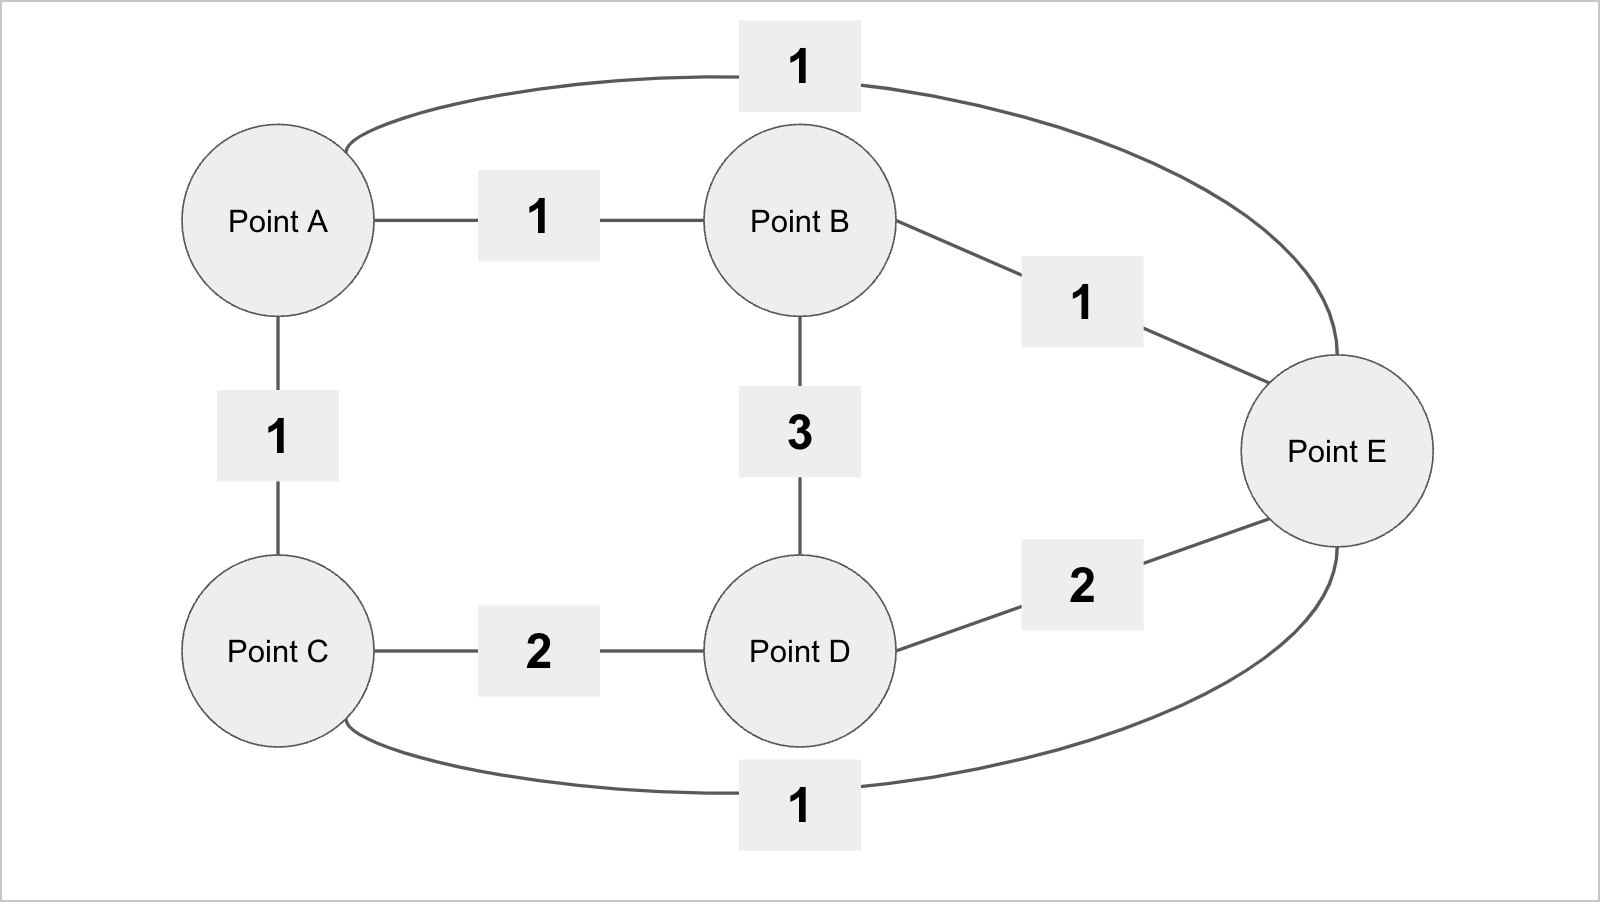
\includegraphics[width=8cm]{./image/03-Tech/chap3/sample_node.png}

\section{ディレクトリ構造}
\begin{tcolorbox}[title=ディレクトリ構造]
    \begin{verbatim}
├── build
│   ├── Docker
│   │   ├── go
│   │   │   └── Dockerfile
│   │   └── neo4j
│   │       ├── Dockerfile
│   │       └── volumes
│   │           ├── import
│   │           │   ├── done
│   │           │   ├── points.csv
│   │           │   └── route.csv
│   │           └── script
│   │               └── import_data.sh
│   └── docker-compose.yml
└── server
    ├── config
    │   ├── config.go
    │   └── environments
    │       └── neo4j.yml
    ├── controllers
    │   └── coordinate_controller.go
    ├── db
    │   └── neo4j.go
    ├── go.mod
    ├── go.sum
    ├── main.go
    ├── models
    │   └── coordinate.go
    ├── router
    │   └── router.go
    └── sample.http
\end{verbatim}
\end{tcolorbox}

\section{Neo4jに最初にインポートするファイル}

\begin{tcolorbox}[title=point.csv]
    \begin{verbatim}
1 point_id:ID,point_name,:LABEL
2 a,PointA,Point;Position
3 b,PointB,Point;Position
4 c,PointC,Point;Position
5 d,PointD,Point;Position
6 e,PointE,Point;Position
\end{verbatim}
\end{tcolorbox}


\begin{tcolorbox}[title=route.csv]
    \begin{verbatim}
:START_ID,:END_ID,:TYPE,cost:int
b,a,Distance,1
c,b,Distance,3
d,c,Distance,2
e,d,Distance,2
c,a,Distance,1
d,a,Distance,2
e,b,Distance,1
e,a,Distance,1
c,e,Distance,1
d,b,Distance,3
a,b,Distance,1
b,c,Distance,3
c,d,Distance,2
d,e,Distance,2
a,c,Distance,1
a,d,Distance,2
b,e,Distance,1
a,e,Distance,1
e,c,Distance,1
b,d,Distance,3
\end{verbatim}
\end{tcolorbox}
これらをNeo4jにインポートすることで、先ほどの図を表現することができます。
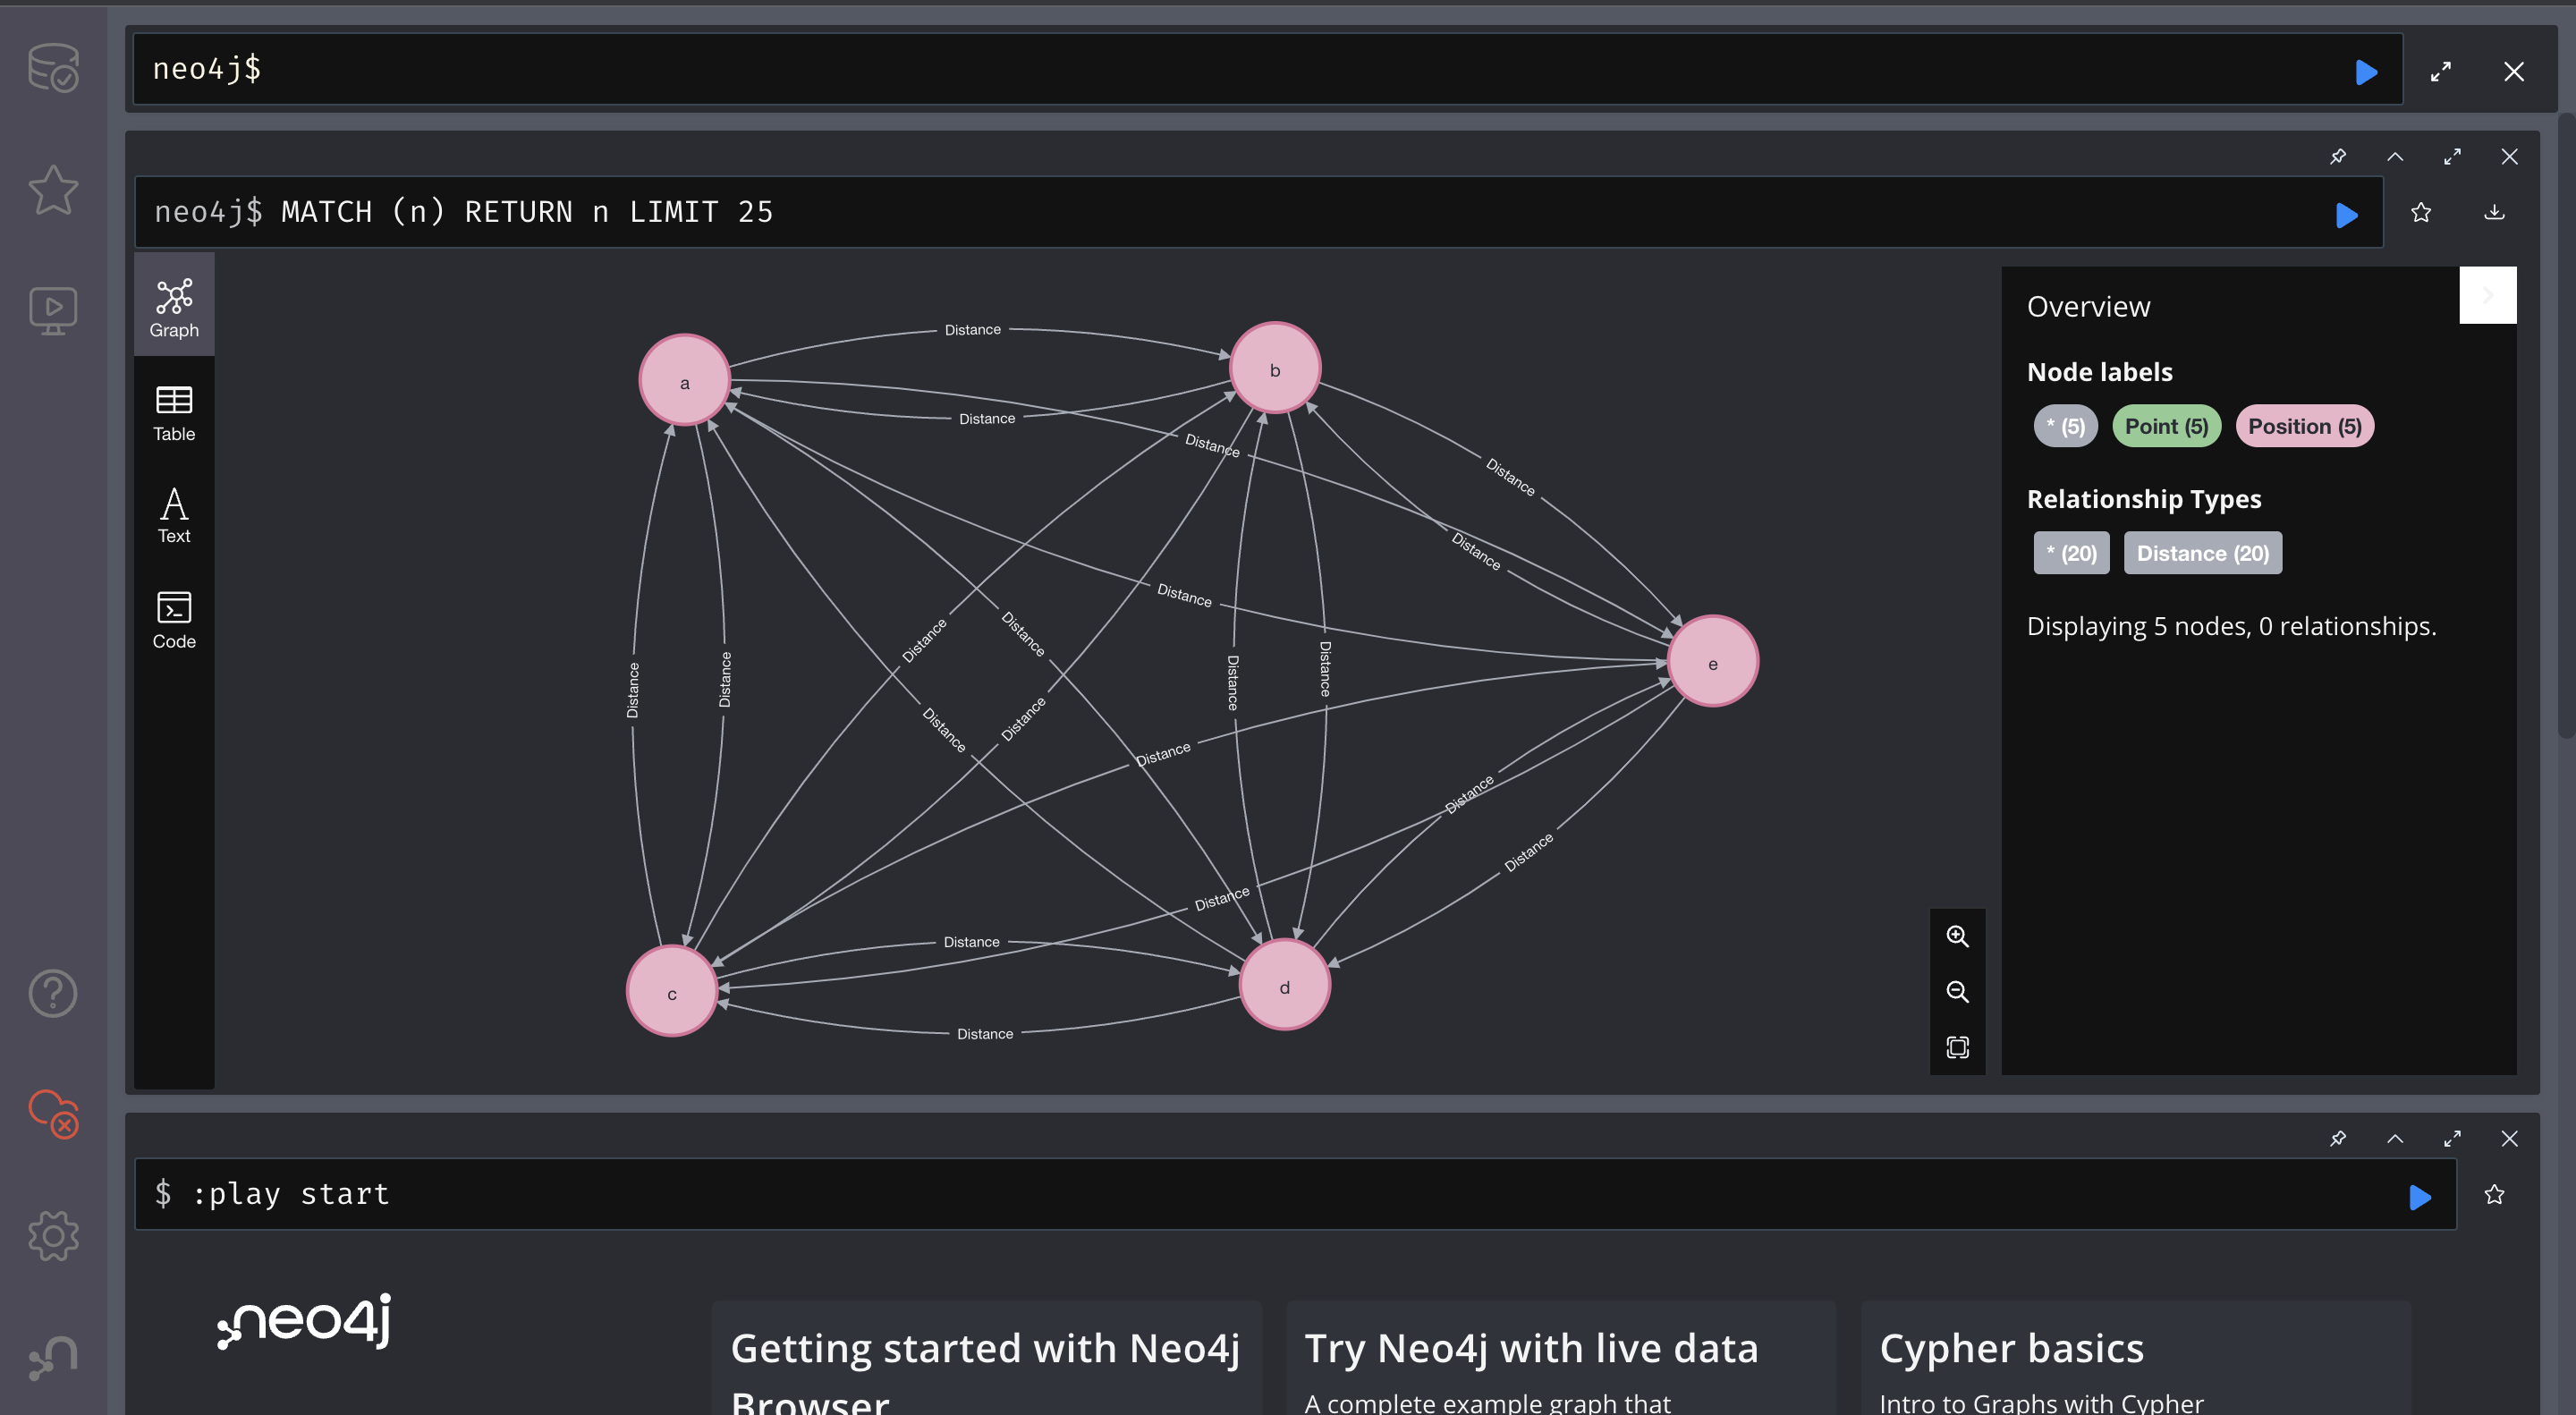
\includegraphics[width=10cm]{./image/03-Tech/chap3/neo4j_result.png}

無事できてますね。

\begin{tcblisting}{title={docker-compose-yml},listing only,breakable, listing options={style=mystyle}}
  1 version: "3"
  2 services:
  3   go:
  4     container_name: NEO4JAPI_GO
  5     build:
  6       context: ./docker/go
  7       dockerfile: Dockerfile
  8     stdin_open: true
  9     tty: true
  10    volumes:
  11      - ../server:/server
  12    ports:
  13      - 8080:8080
  14    networks:
  15      app_net:
  16        ipv4_address: 192.168.0.1
  17    depends_on:
  18      - "neo4j"
  19
  20  neo4j:
  21    container_name: NEO4JAPI_NEO4J
  22    build:
  23      context: ./Docker/neo4j
  24      dockerfile: Dockerfile
  25    restart: always
  26    ports:
  27      - 57474:7474
  28      - 57687:7687
  29    volumes:
  30      - ./Docker/neo4j/volumes/data:/data
  31      - ./Docker/neo4j/volumes/logs:/logs
  32      - ./Docker/neo4j/volumes/conf:/conf
  33      - ./Docker/neo4j/volumes/import:/import
  34      - ./Docker/neo4j/volumes/script:/script
  35    environment:
  36      - NEO4J_AUTH=neo4j/admin
  37      - EXTENSION_SCRIPT=/script/import_data.sh
  38    networks:
  39      app_net:
  40        ipv4_address: 192.168.0.2
  41
  42 networks:
  43  app_net:
  44    driver: bridge
  45    ipam:
  46      driver: default
  47      config:
  48        - subnet: 192.168.0.0/24
\end{tcblisting}


volumesはデータベースに入れるデータ、ログをバインドするための場所を指定しています。
environmentではユーザーとパスワード、最初に読み込んでもらうシェルスクリプトの場所を指定します。

go関連のDockerfile。
\begin{tcolorbox}[title=Dockerfile]
\begin{verbatim}

1  # goバージョン
2  FROM golang:1.19.3-alpine
3  # アップデートとgitのインストール
4  RUN apk add --update &&  apk add git
5  # appディレクトリの作成
6  RUN mkdir /server
7  # ワーキングディレクトリの設定
8  WORKDIR /server
9  # ホストのファイルをコンテナの作業ディレクトリに移行
10 ADD . /server
11 # main.goを実行
12 CMD ["go", "run", "main.go"]
\end{verbatim}
\end{tcolorbox}

Neo4j関連のDockerfile。
\begin{tcolorbox}[title=Dockerfile]
\begin{verbatim}
1  # goバージョン
2  FROM golang:1.19.3-alpine
3  # アップデートとgitのインストール
4  RUN apk add --update &&  apk add git
5  # appディレクトリの作成
6  RUN mkdir /server
7  # ワーキングディレクトリの設定
8  WORKDIR /server
9  # ホストのファイルをコンテナの作業ディレクトリに移行
10 ADD . /server
11 # main.goを実行
12 CMD ["go", "run", "main.go"]
\end{verbatim}
\end{tcolorbox}

csvファイルを読ませるためのシェルスクリプト。
\begin{tcolorbox}[title=import\_data.sh]
\begin{verbatim}
1  #!/bin/bash
2  set -euC
3
4  # EXTENSION_SCRIPTはコンテナが起動するたびにコールされるため、
5  # import処理が実施済かフラグファイルの有無をチェック
6  if [ -f /import/done ]; then
7      echo "Skip import process"
8      return
9  fi
10
11 # データを全削除
12 echo "delete database started."
13 rm -rf /data/databases
14 rm -rf /data/transactions
15 echo "delete database finished."
16
17 # CSVデータのインポート
18 echo "Start the data import process"
19 neo4j-admin import \
20   --nodes=/import/points.csv \
21   --relationships=/import/route.csv
22 echo "Complete the data import process"
23
24 # import処理の完了フラグファイルの作成
25 echo "Start creating flag file"
26 touch /import/done
27 echo "Complete creating flag file"
\end{verbatim}
\end{tcolorbox}
    
\section{Goのソースコード}
\subsection{configディレクトリ}

\begin{tcolorbox}[title=config.go]
\begin{verbatim}
1  package config
2
3  import (
4  	  "github.com/spf13/viper"
5  )
6
7  var n *viper.Viper
8
9  func init() {
10 	 n = viper.New()
11	 n.SetConfigType("yaml")
12 	 n.SetConfigName("neo4j")
13 	 n.AddConfigPath("config/environments/")
14 }
15
16 func GetNeo4jConfig() *viper.Viper {
17	 if err := n.ReadInConfig(); err != nil {
18		 return nil
19	 }
20	 return n
21 }
\end{verbatim}
\end{tcolorbox}
このファイルでneo4j.yamlの環境変数を読み込みます。
\begin{tcolorbox}[title=neo4j.yml]
\begin{verbatim}
1 neo4j:
2  user: neo4j
3  password: admin
4  uri: neo4j://192.168.176.1:57687
\end{verbatim}
\end{tcolorbox}
Neo4jと接続するための環境変数です。

\subsection{dbディレクトリ}





\begin{tcblisting}{title={neo4j.go},listing only,breakable, listing options={style=mystyle}}
1  package db
2
3  import (
4   "log"
5
6   "neo4japi/server/config"
7
8   "github.com/neo4j/neo4j-go-driver/v4/neo4j"
9  )
10
11 func GetDriverAndSession() neo4j.Session {
12   n := config.GetNeo4jConfig()
13   dr, err := neo4j.NewDriver(n.GetString("neo4j.uri"), neo4j.BasicAuth(n.GetString("neo4j.user"), n.GetString("neo4j.password"), ""))
14   if err != nil {
15     log.Fatal(err)
16   }
17   ses := dr.NewSession(neo4j.SessionConfig{AccessMode: neo4j.AccessModeRead})
18   return ses
19 }
  \end{tcblisting}
  
このファイルでNeo4jと接続し、セッションを返すようにします。
\subsection{modelsディレクトリ}


\begin{tcblisting}{title={coordinate.go},listing only,breakable, listing options={style=mystyle}}
  1  package models
  2
  3  import (
  4   "fmt"
  5   "log"
  6
  7   "neo4japi/server/db"
  8
  9   "github.com/neo4j/neo4j-go-driver/v4/neo4j"
  10 )
  11
  12 type Route struct {
  13   Position string `json:"point"`
  14 }
  15
  16 func FindRoute(fr, to string) []*Route {
  17   var r []*Route
  18   ses := db.GetDriverAndSession()
  19   defer ses.Close()
  20   cyp := fmt.Sprintf(`
  21     MATCH (from:Position {point_name: "%s"}), (to:Position {point_name: "%s"}), 
  22       path=allShortestPaths ((from)-[distance:Distance*]->(to))
  23     WITH
  24       [position in nodes(path) | position.point_name] as name,
  25     REDUCE(totalMinutes = 0, d in distance | totalMinutes + d.cost) as 所要時間
  26     RETURN name
  27     ORDER BY 所要時間
  28     LIMIT 10;
  29   `, fr, to)
  30
  31   _, err := ses.ReadTransaction(func(transaction neo4j.Transaction) (interface{}, error) {
  32     result, err := transaction.Run(cyp, nil)
  33     if err != nil {
  34       return nil, err
  35     }
  36     if result.Next() {
  37       name, _ := result.Record().Get("name")
  38       nameAr := name.([]interface{})
  39
  40       for i := 0; i < len(nameAr); i++ {
  41         r = append(r, &Route{nameAr[i].(string)})
  42      }
  43     }
  44     return nil, result.Err()
  45   })
  46   if err != nil {
  47     log.Fatal(err)
  48   }
  49   return r
  50 }
    \end{tcblisting}



出発地点と目的地を受け取ることでNeo4jにCypherというクエリ言語を用いて最短経路を導出してもらいます。
\subsection{controllersディレクトリ}

\begin{tcolorbox}[title=coordinate\_controller.go]
\begin{verbatim}
1  package controllers
2
3  import (
4	  "net/http"
5
6	  "github.com/gin-gonic/gin"
7	  "neo4japi/server/models"
8  )
9
10 func RouteSearch(c *gin.Context) {
11	 fr := c.Query("fr")
12	 to := c.Query("to")
13	 res := models.FindRoute(fr, to)
14	 c.JSON(http.StatusOK, res)
15 }
\end{verbatim}
\end{tcolorbox}
GETリクエストで受け取ったパラメータを models で作成した関数に渡します。
\subsection{routerディレクトリ}

\begin{tcolorbox}[title=router.go]
\begin{verbatim}
1  package router
2
3  import (
4	  "github.com/gin-gonic/gin"
5	  "neo4japi/server/controllers"
6  )
7
8  func Init() {
9	  r := gin.Default()
10	 r.GET("/coordinate", controllers.RouteSearch)
11	 r.Run()
12 }
\end{verbatim}
\end{tcolorbox}
ルーティング先を定義します。
\subsection{実行ファイル}
\begin{tcolorbox}[title=coordinate\_controller.go]
\begin{verbatim}
1  package main
2
3  import (
4	  "neo4japi/server/router"
5  )
6
7  func main() {
8	  router.Init()
9  }
\end{verbatim}
\end{tcolorbox}

\section{実行方法}
\begin{tcolorbox}[breakable]
\begin{verbatim}
docker compose up
\end{verbatim}
\end{tcolorbox}
このコマンドを実行することで Neo4j サーバーと Gin サーバーが立ち上がります。
\subsection{実行確認}

\begin{tcolorbox}[title=sample.http]
\begin{verbatim}
1  GET http://localhost:8080/coordinate?fr=PointB&to=PointE
\end{verbatim}
\end{tcolorbox}
今回はVSCodeの拡張機能であるREST Clientを用いて実行確認を行います。

ここで、 coordinate?fr=PointB\&to=PointE の部分を自分の好きな地点にしてリクエストを送ると、最短経路が返されます。

\section{おわりに}
このチャプターではグラフDBとGo言語を用いたAPIサーバーの建て方を説明しました。
Gin、Neo4jは奥が深いので、もし気になった方はぜひ自分で調べて触ってみてください。
